% ----------------------------------------------------------------------------
% Setup and configuration
% ----------------------------------------------------------------------------

\documentclass{article}
\usepackage[utf8]{inputenc}

% for serious mathematical typesetting, https://www.ctan.org/pkg/amsmath
\usepackage{amsmath}

% use H to place figures and tables at exact location, https://www.ctan.org/pkg/float
\usepackage{float}

% manage images and define the images folder, https://ctan.org/pkg/graphicx
\usepackage{graphicx}
\graphicspath{{figures/}}

% create hyperlinks in the document and disable border, https://ctan.org/pkg/hyperref
\usepackage[hidelinks]{hyperref}

% greek letters in text without math mode, https://www.ctan.org/pkg/textgreek
\usepackage{textgreek}

% bibliography package and references file, https://www.ctan.org/pkg/biblatex
\usepackage{biblatex}
\addbibresource{references.bib}

% ----------------------------------------------------------------------------
% Document
% ----------------------------------------------------------------------------

\title{Modeling Gas Effects in a Bubbling Fluidized Bed Reactor for Biomass Pyrolysis}
\author{Gavin M. Wiggins, ??}
\date{\today}

\begin{document}

\maketitle
\tableofcontents

%!TEX root = ../main.tex

\section*{Abstract}

Fast pyrolysis of biomass in a fluidized bed reactor is typically conducted in a nitrogen gas environment. Recycling product gas can improve the economics of operating such a system by reducing reliance on pure process streams.

%!TEX root = ../main.tex

\section{Introduction}

Fast pyrolysis is a versatile method for thermochemical conversion of solid biomass into liquid bio-oil which can be used for bio-fuel and high-value chemical production. Bio-oil is commonly generated in bubbling fluidized bed and circulating fluidized bed reactor systems in which biomass particles rapidly devolatilize in the absence of oxygen into mixtures of light gases, condensable bio-oil vapors, and solid char \cite{Bridgwater-1999, Bridgwater-2018a, Mohan-2006}. Since biomass pyrolysis normally occurs in a non-oxidizing environment, the fluidization gas (carrier gas) is often pure nitrogen \cite{Mohan-2006}. To maximize bio-oil yields, the reactor typically operates at temperatures near 500$^\circ$C and must maintain particle residence times up to 10 seconds and gas residence times less than 2 seconds \cite{Bridgwater-2018a}. Deviations from these conditions can result in significant production and quality penalties; therefore, optimal reactor design and control become crucial to achieving commercially viable bio-oil production.

To improve the economic feasibility of biomass fast pyrolysis systems, char can be burned for process heat while recycled pyrolysis gas can assist with fluidization \cite{Bridgwater-1999, Mante-2012}. The major generated components of pyrolysis gas are CO, CO$_2$, CH$_4$, H$_2$, along with other light hydrocarbons \cite{Asadullah-2008, Zhang-2011}. Several experiments investigated the effects of these gases on reactor conditions and pyrolysis yields \cite{Mante-2012, Mullen-2013, Zhang-2011} but modeling the effects of the different gases was not discussed.

Autothermal pyrolysis experiments in a fluidized bed reactor has shown that the presence of oxygen in the carrier gas can prevent reactor clogging by reducing char formation \cite{Kim-2014}. The addition of oxygen can also improve heat transfer within the reactor via partial oxidiation of the pyrolysis products without significant decreases in bio-oil yield \cite{Polin-2019a}. Substituting air for nitrogen gas allowed for higher superficial velocities which promoted elutriation of char from reactor experiments while having neglible effect on bio-oil yield \cite{Polin-2019b}. Modeling the fluidization of the autothermal experiments was not discussed in the available literature.

There are several fluidized bed reactor models that investigate the hydrodynamics and conversion of biomass at fast pyrolysis conditions \cite{Papadikis-2009, Papadikis-2010, Mellin-2014, Xiong-2016, Xue-2011}. These models assume the carrier gas is pure nitrogen which is a typical scenario for biomass fast pyrolysis. The authors are not aware of any models in the biomass pyrolysis literature that investigate the effects of a carrier gas other than pure nitrogen. Consequently, our objective in this paper is to evaluate different fluidization gases and their effects on the hydrodynamics and biomass conversion in a fluidization bed reactor operating at fast pyrolysis conditions. Our methodology uses engineering correlations, reducing-order modeling techniques, and CFD simulations to model these effects and compare the model results (where applicable) to experimental data.

%!TEX root = ../main.tex

\section{Experimental apparatus}

The NREL 2FBR reactor system thermochemically converts biomass feedstock at fast pyrolysis conditions. The system is comprised of two bubbling fluidized bed (BFB) reactors where the first reactor is for biomass fast pyrolysis and the second reactor is for vapor phase upgrading. Yields from the BFB pyrolysis reactor are compared to model results discussed later in this paper.

An overview of the NREL 2FBR system is shown in Figure \ref{fig:nrel-system}, components of the pyrolysis reactor are detailed in Figure \ref{fig:pyrolyzer-components}, while dimensions and typical operating conditions of the pyrolysis unit are given in Figure \ref{fig:pyrolyzer-dims-flows}. Sand is used as the dominant heat transfer medium in the pyrolyzer. Biomass particles are fed to the reactor via a screw auger and nitrogen is used as the fluidization/carrier gas. More information about the NREL 2FBR biomass pyrolysis system is available elsewhere \cite{Howe-2015, Trendewicz-2015}.

\begin{figure}[H]
    \centering
    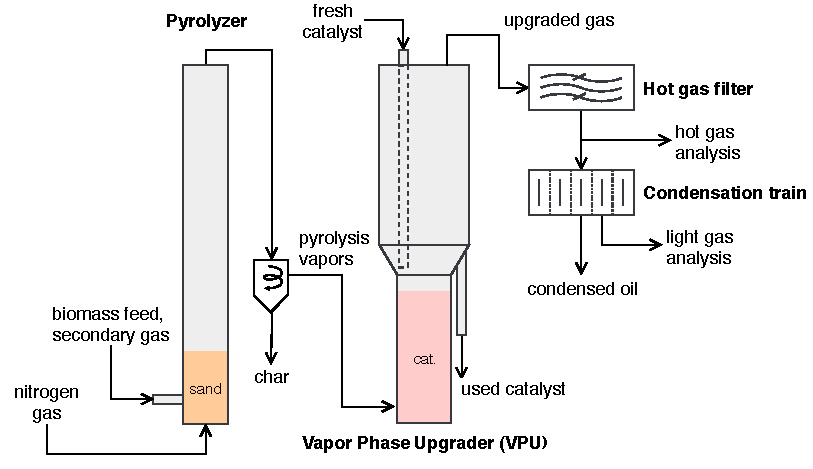
\includegraphics[width=0.8\textwidth]{system.pdf}
    \caption{Overview of the NREL 2FBR system. Biomass fast pyrolysis occurs in the pyrolyzer (left) and gaseous products are catalytically upgraded in the vapor phase upgrader (right).}
    \label{fig:nrel-system}
\end{figure}

\begin{figure}[H]
    \centering
    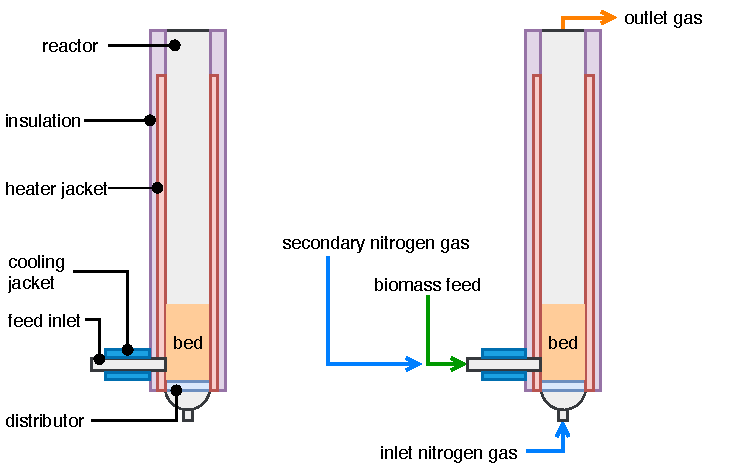
\includegraphics[width=0.8\textwidth]{pyrolyzer-components.pdf}
    \caption{Components of the BFB biomass pyrolysis reactor referred to as the ``pyrolyzer'' in the NREL 2FBR system.}
    \label{fig:pyrolyzer-components}
\end{figure}

\begin{figure}[H]
    \centering
    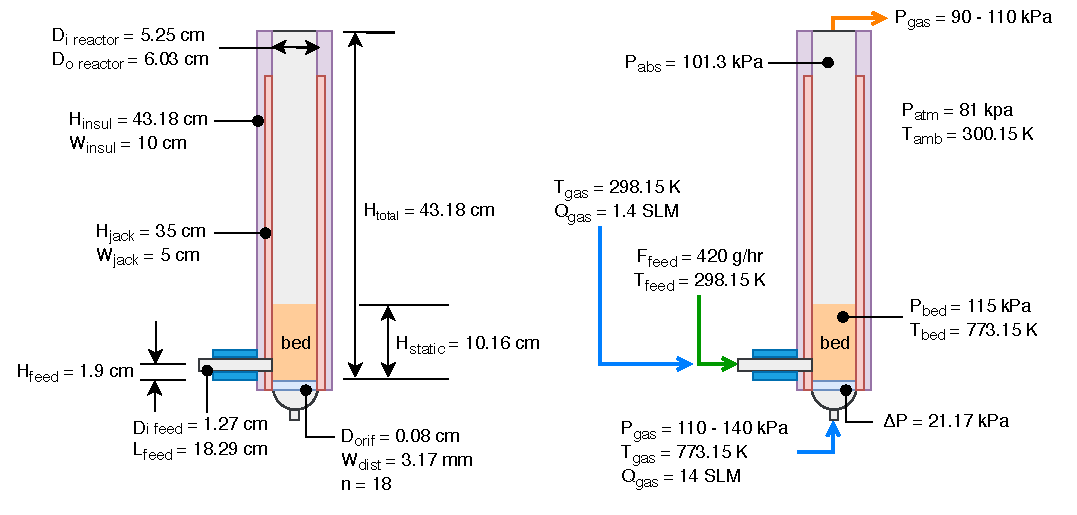
\includegraphics[width=\textwidth]{pyrolyzer-dims-flows.pdf}
    \caption{Dimensions and typical fast pyrolysis operating conditions for the BFB biomass pyrolysis reactor in the NREL 2FBR system.}
    \label{fig:pyrolyzer-dims-flows}
\end{figure}

%!TEX root = ../main.tex

\section{Modeling approach}

Our strategy to model gas effects in a bubbling fluidized bed reactor begins with determining gas properties such as density, dynamic viscosity, thermal conductivity, and heat capacity. Once the individual gas viscosity is known, the viscosity of a gas mixture is calculated using various mixture models. Next, fluidization correlations relevant to fluidized bed reactors are used to investigate the effects of the gas properties on the hydrodynamics of the system. Dimensionless numbers provide insight on the limiting mechanisms in regards to the pyrolysis of the biomass particles. Finally, CFD-DEM simulations provide residence times and product yields related to the different carrier gas properties.

% ----------------------------------------------------------------------------

\subsection{Gas properties}

Gas density is calculated using the ideal gas law as shown in Equation \ref{eq:density} where $\rho_\text{gas}$ is density in kg/m$^3$, P is pressure in Pa, M is molecular weight as g/mol, R is the gas constant in units of (m$^3$ Pa) / (K mol), and T is temperature in Kelvin.

\begin{equation}\label{eq:density}
    \rho_\text{gas} = \frac{P\,M}{R\,T}
\end{equation}

Dynamic gas viscosity $\mu_\text{gas}$ is estimated by Equation \ref{eq:viscosity} in units of \textmugreek P. Gas thermal conductivity k$_\text{gas}$ as W/m\,K is calculated from Equation \ref{eq:thermlcond} and heat capacity C$_\text{p\,gas}$ as J/mol\,K is determined using Equation \ref{eq:heatcap}. Temperature is denoted by T in Kelvin while the regression coefficients A, B, C, D, E, F, and G for a particular gas are obtained from Yaws' Handbook \cite{Yaws2014}.

\begin{equation}\label{eq:viscosity}
    \mu_\text{gas} = A + B\,T + C\,T^2 + D\,T^3
\end{equation}

\begin{equation}\label{eq:thermlcond}
    k_\text{gas} = A + B\,T + C\,T^2 + D\,T^3
\end{equation}

\begin{equation}\label{eq:heatcap}
    C_\text{p\,gas} = A + B\,T + C\,T^2 + D\,T^3 + E\,T^4 + F\,T^5 + G\,T^6
\end{equation}

Several methods are available to calculate the dynamic viscosity of a gas mixture. The simplest approach is Graham's model in Equation \ref{eq:graham} which sums the gas viscosities $\mu_\text{i}$ and mole fractions x$_\text{i}$ of each gas component \cite{Graham-1846}.

\begin{equation}
    \mu_\text{mix} = \sum(x_i \; \mu_i)
    \label{eq:graham}
\end{equation}

\noindent The Herning and Zipperer approach shown by Equation \ref{eq:herning}, sums the viscosities weighted by the square root of the molecular weight M$_\text{i}$ for each component \cite{Herning-1936}. According to Davidson's report \cite{Davidson-1993}, this model is not recommended for gas mixtures containing significant amounts of hydrogen.

\begin{equation}
    \mu_\text{mix} = \sum \frac{\mu_i \; x_i \; \sqrt{M_i}}{x_i \; \sqrt{M_i}}
    \label{eq:herning}
\end{equation}

\noindent Wilke's model represented by Equations \ref{eq:wilke-phi} and \ref{eq:wilke-mu} is based on a kinetic theory implementation which requires a coefficient $\phi_\text{ij}$ for each gas component \cite{Wilke-1950}. The coefficients are used along with the mole fractions to calculate the overall mixture viscosity.

\begin{align}
    \phi_{ij} &= \frac{\left[1 + (\mu_i/\mu_j)^{1/2} (M_j/M_i)^{1/4}\right]^2}{(4/\sqrt{2}) \left[1 + (M_i/M_j)\right]^{1/2}} \label{eq:wilke-phi} \\
    \mu_{\text{mix}} &= \sum_{i=1} \frac{\mu_i}{1 + \frac{1}{x_i} \sum_{\substack{j=1 \\j \neq i}} x_j \, \phi_{ij}} \label{eq:wilke-mu}
\end{align}

\noindent Brokaw provides a model for nonpolar and polar gas mixtures that utilizes the viscosities, molecular weights, and mole fractions of the mixture components \cite{Brokaw-1968}. The molecular weight ratios of the gas components are described by Equations \ref{eq:brokaw-mij} and \ref{eq:brokaw-aij}; the ratios are used in Equation \ref{eq:brokaw-mu} to calculate the overall mixture viscosity where S$_\text{ij} = 1$ for nonpolar gases.

\begin{align}
    m_{ij} &= \left[ 4 M_i M_j / (M_i + M_j)^2 \right]^{1/4} \label{eq:brokaw-mij} \\
    A_{ij} &= m_{ij}\left( \frac{M_j}{M_i} \right)^{1/2} \left[ 1 + \frac{\frac{M_i}{M_j} - \left(\frac{M_i}{M_j} \right)^{0.45} }{ 2 \left(1 + \frac{M_i}{M_j} \right) + \frac{1 + \left(\frac{M_i}{M_j} \right)^{0.45}}{1 + m_{ij}} m_{ij}} \right] \label{eq:brokaw-aij} \\
    \mu_{\text{mix}} &= \sum_{i=1} \frac{x_i \sqrt{\mu_i}}{\frac{x_i}{\sqrt{\mu_i}} + \sum_{\substack{j=1 \\ j \neq i}} \frac{S_{ij} \, A_{ij}}{\sqrt{\mu_j}} x_j} \label{eq:brokaw-mu}
\end{align}

\noindent Lastly, the approach by Davidson estimates viscosity in terms of the fluidity of the gas mixture \cite{Davidson-1993}. This method utilizes the momentum efficiency of the gas components to predict the mixture fluidity which is the reciprocal of the gas viscosity as given by Equations \ref{eq:davidson-eij}, \ref{eq:davidson-f}, and \ref{eq:davidson-mu} respectively. The empirical constant A was calculated as 0.375 using reported viscosities of 35 gas pairs \cite{Davidson-1993}.

\begin{align}
    E_{ij} &= \frac{2 \sqrt{M_i\, M_j}}{M_i + M_j} \label{eq:davidson-eij} \\
    f &= \sum \frac{x_i\, x_j}{\sqrt{\mu_i\, \mu_j}} E_{ij}^A \label{eq:davidson-f} \\
    \mu_\text{mix} &= 1 / f \label{eq:davidson-mu}
\end{align}

% ----------------------------------------------------------------------------

\subsection{Fluidization correlations}

For a bed of particles, the minimum fluidization velocity U$_\text{mf}$ is the gas velocity at which the drag force of the upward moving gas equals the weight of the particles. Kunii and Levenspiel \cite{Levenspiel-1991} provide the following equation for calculating minimum fluidization velocity

\begin{equation}
    U_\text{mf} = \frac{Re_\text{p,mf}\; \mu}{d_p\, \rho_g}
\end{equation}

\noindent where $\mu$ is gas viscosity in kg/m\,s, d$_\text{p}$ is particle diameter in meters, $\rho_\text{g}$ is gas density in kg/m$^3$, and Re$_\text{p,mf}$ is the particle Reynolds number at minimum fluidization conditions. The Reynolds number is calculated using the Archimedes number (Ar) as follows

\begin{align}
    Re_{p,mf} &= \left( a^2 + b Ar \right)^{1/2} - a \\
    Ar &= \frac{d_p^3 \rho_g (\rho_s - \rho_g) g}{\mu^2}
\end{align}

\noindent where a and b are dimensionless constants which represent experimental coefficients. Some U$_\text{mf}$ correlations in the literature are based on experimental data from Wen and Yu where a, b = 33.7, 0.0408; from Richardson where a, b = 25.7, 0.0365; and from Grace where a, b = 27.2, 0.0408 \cite{Levenspiel-1991}. However, Kunii and Levenspiel \cite{Levenspiel-1991} suggest the constants ($a, b$) can be derived from the Ergun pressure drop equation based on constants K$_1$ and K$_2$ where $\epsilon_\text{mf}$ is the bed void fraction at minimum fluidization and $\phi$ is sphericity of the bed particles. For this paper, U$_\text{mf}$ is estimated based on the Ergun, Grace, Richardson, and Wen and Yu correlations.

\begin{equation}
    a = \frac{K_2}{2 K_1} \qquad
    b = \frac{1}{K_1}
\end{equation}

\begin{equation}
    K_1 = \frac{1.75}{\epsilon_{mf}^3 \phi} \qquad
    K_2 = \frac{150(1-\epsilon_{mf})}{\epsilon_{mf}^3 \phi^2}
\end{equation}

The terminal velocity of particles, U$_\text{t}$, is the minimum gas velocity to necessary to entrain a particle of size d$_\text{p}$ in the flow. This velocity can be estimated from the maximum velocity of a particle in free-fall through a fluid, which is given by Equation \ref{eq:terminal}. Here, Re$_\text{p}$ is the particle Reynolds number given by Equation \ref{eq:particleRe} and C$_\text{D}$ is the drag coefficient, which can be estimated from an emperical correlation developed by Haider and Levenspiel \cite{haider1989drag} and given by Equation \ref{eq:dragCoeff}.

\begin{align}
    U_{t} &= \left [\frac{4d_{p} \left (\rho_{s}-\rho_{g} \right )g}{3\rho_{g}C_{D}}\right ]^{1/2} \label{eq:terminal} \\
    Re_{p} &= \frac{d_{p}U_{t}\rho_{g}}{\mu_{g}} \label{eq:particleRe} \\
    C_{D} &= \frac{24}{Re_{p}}\left [ 1+\left ( 8.1716e^{-4.0655\phi } \right )Re_{p}^{0.0964+0.5565\phi} \right ]+\frac{73.69Re_{p}e^{-5.0748\phi}}{Re_{p}+5.378e^{6.2122\phi}} \label{eq:dragCoeff}
\end{align}


% based on results, it looks like h is a function of Umf and not U, so this was changed back
As shown in Equation \ref{eq:nusselt}, the convective heat transfer coefficient h in units of W/m$^2$K can be determined from the Nusselt number Nu where Re is the Reynolds number, d$_\text{p}$ is the biomass particle diameter, d$_\text{b}$ is the sand particle diameter, and k$_\text{g}$ is the gas thermal conductivity in W/m\,K. This approach is valid for $\text{d}_\text{p} < \text{d}_\text{b}$ \cite{Collier-2004}. The Reynolds number is determined from $\rho$ which is the gas density in kg/m$^3$, the minimum fluidization velocity U$_\text{mf}$ in m/s, and the dynamic gas viscosity $\mu$ in kg/m\,s \cite{Papadikis-2010}.

\begin{align}
    Nu &= 2 + 0.9\, Re^{0.62} \left(\frac{d_p}{d_b}\right)^{0.2} = \frac{h\, d_p}{k_g} \label{eq:nusselt} \\
    Re &= \frac{\rho\, U_{mf}\, d_p}{\mu}
\end{align}

% ----------------------------------------------------------------------------

\subsection{Dimensionless numbers}

As mentioned in the work of Pyle and Zaror \cite{Pyle-1984}, the rate of pyrolysis involves a balance between internal and external heat transfer due to heat transport and reaction. This balance is embodied by the dimensionless numbers Bi, Py$^\text{I}$, and Py$^\text{II}$ which are determined from Equations \ref{eq:biot}, \ref{eq:pynumber1}, and \ref{eq:pynumber2} respectively. The Biot number Bi represents the ratio of convective and conductive heat transport. The first pyrolysis number Py$^\text{I}$ demonstrates the ratio of heat transfer by conduction to the rate of heat loss due to products leaving the particle. The second pyrolysis number Py$^\text{II}$ is the effect of convective heat transfer to the external particle surface relative to the reaction heat loss. The Biot and pyrolysis numbers are calculated using the following parameters: h is the convective heat transfer coefficient in W/m$^2$K, R is the radius or characteristic length of the biomass particle in meters, k is the biomass thermal conductivity in W/mK, $\rho$ is the density of the biomass particle in kg/m$^3$, K is the total rate constant in 1/s for the primary reactions, and C$_\text{p}$ is the biomass heat capacity calculated from $103.1 + 3.867\,\text{T}$ where T is the biomass temperature in Kelvin.

\begin{align}
    Bi &= \frac{h\,R}{k} \label{eq:biot} \\
    Py^{\textrm{I}} &= \frac{k}{\rho\,C_p\,R^2\,K} \label{eq:pynumber1} \\
    Py^{\textrm{II}} &= \frac{h}{\rho\,C_p\,R\,K} \label{eq:pynumber2}
\end{align}

The Prandtl number is a dimensionless number representing the ratio of momentum diffusivity to thermal diffusivity. It is calculated from the equation shown below where C$_\text{p}$ is heat capacity (J/kg$\cdot$K), $\mu$ is dynamic gas viscosity (kg/m$\cdot$s), and k is thermal conductivity (W/m$\cdot$K).

\begin{equation}
    Pr = \frac{C_p\, \mu}{k}
\end{equation}

% ----------------------------------------------------------------------------

\subsection{Biomass pyrolysis kinetics}

A pyrolysis kinetics scheme based on the work of Di Blasi was implemented to predict the conversion of biomass into gas, tar, and char products \cite{Blasi-1993,Blasi-2001}. Figure \ref{fig:blasi} gives an overview of the scheme and its reaction mechanisms. Reactions 1--3 represent the primary conversion of biomass while reactions 4--5 are secondary reactions that reduce tar yield at long residence times. Reaction 6 is the conversion of moisture in the biomass to water vapor.

\begin{figure}[H]
    \centering
    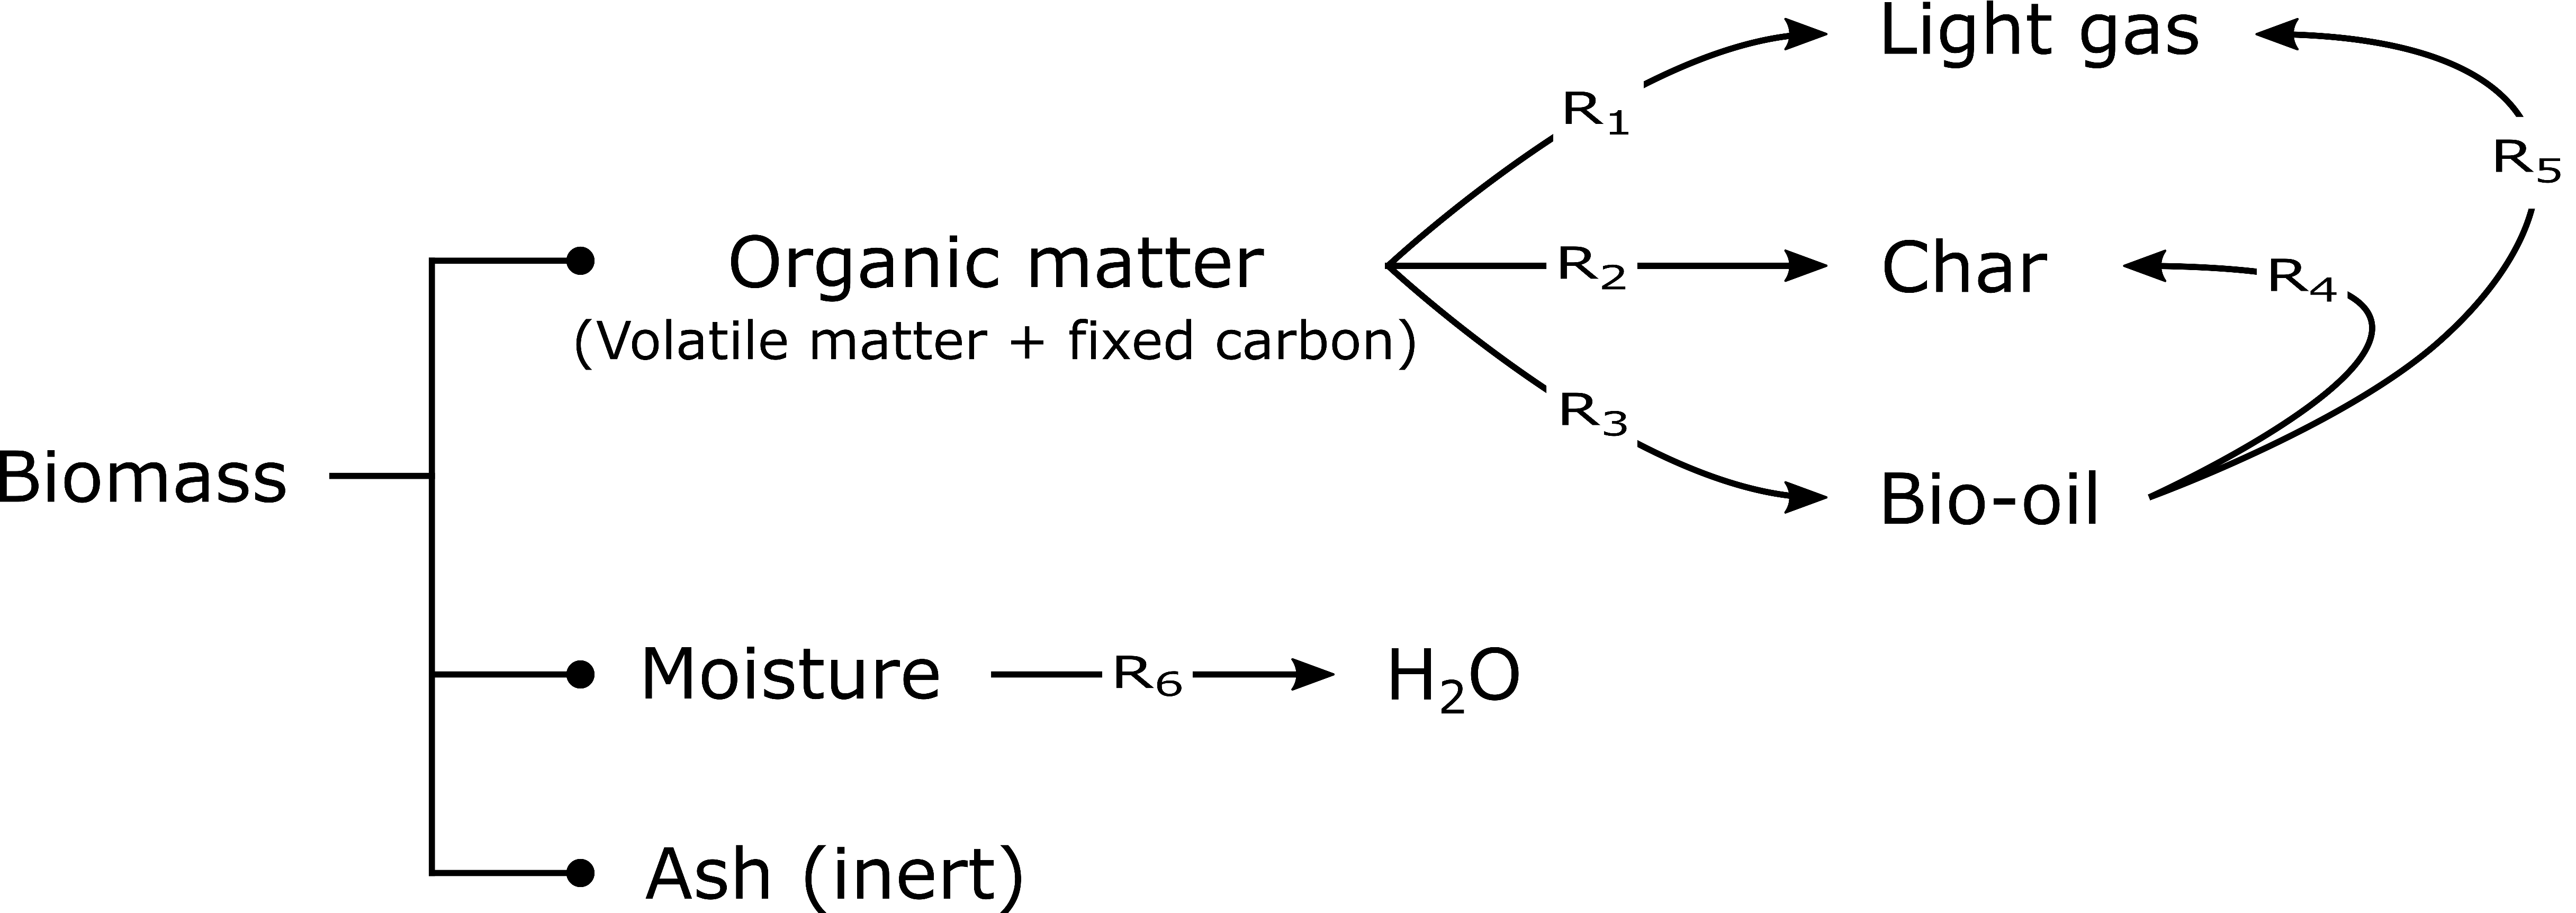
\includegraphics[width=0.8\textwidth]{kinetics.pdf}
    \caption{Diagram of the Di Blasi pyrolysis kinetics scheme for conversion of biomass to gas, tar, and char products.}
    \label{fig:blasi}
\end{figure}

The pyrolysis reactions were modeled as first-order Arrhenius type equations where the reaction rate is given as

\begin{equation}
    r_i = C_i\,A_i\,e^{-E_i / R\,T}
\end{equation}

\noindent where r$_\text{i}$ is the rate of reaction i such that C$_\text{i}$ is a mass based concentration, A$_\text{i}$ is the pre-factor (1/s), E$_\text{i}$ is the activation energy (kJ/mol), R is the gas constant, and T is the reaction temperature (K). Kinetic parameters for each reaction are listed in Table \ref{tab:kinetic-params} where $\Delta$H is the heat of reaction (kJ/kg). Based on the work performed by Lu et. al.\cite{lu2020bridging}, which found that the Di Blasi kinetics scheme overpredicts light gas production when using a coarse-grained DEM model, the pre-factor of reaction 4 was modified by a factor 0.2. The value of this factor was determined by comparisons with experiments.

\begin{table}[H]
    \centering
    \caption{Kinetic parameters for the Di Blasi biomass pyrolysis scheme.}
    \begin{tabular}{clrrc}
        \toprule
        Reaction    & A (1/s)               & E (kJ/mol) & $\Delta$H (kJ/kg) & Reference \\
        \midrule
        1           & $4.38 \times 10^9$    & 152.7      & -20               & \cite{Blasi-2001} \\
        2           & $3.27 \times 10^6$    & 111.7      & -20               & \cite{Blasi-2001} \\
        3           & $1.08 \times 10^{10}$ & 148.0      & 255               & \cite{Blasi-2001} \\
        4           & $0.2\left( 4.28 \times 10^6 \right)$    & 108.0      & -42               & \cite{Blasi-1993,lu2020bridging} \\
        5           & $1.00 \times 10^6$    & 108.0      & -42               & \cite{Blasi-1993} \\
        6           & $5.13 \times 10^6$    & 87.6       & 2700              & ? \\
        \bottomrule
    \end{tabular}
    \label{tab:kinetic-params}
\end{table}

% ----------------------------------------------------------------------------

\subsection{CFD-DEM simulation}

A coarse-grained CFD-DEM model was implemented for biomass pyrolysis in MFiX, an open-source, Fortran-based code \cite{Syamlal-1993}. The coarse-grained CFD-DEM model used in this work is an extension of the standard MFiX release. Gas phase transport was described using conservation equations of mass, momentum, energy, and chemical species in the Eulerian framework (Equations \ref{eq:gas-trans-mass}--\ref{eq:gas-trans-chemical}, respectively).

\begin{align}
    \frac{d(\epsilon_g \rho_g)}{dt} + \nabla (\epsilon_g \rho_g u_g) &= S_\rho \label{eq:gas-trans-mass} \\
    \frac{d(\epsilon_g \rho_g u_g)}{dt} + \nabla (\epsilon_g \rho_g u_g u_g) &= -\epsilon_g \nabla p + \nabla (\epsilon_g \tau) + \epsilon_g \rho_g g + S_u \\
    \frac{d(\epsilon_g \rho_g E)}{dt} + \nabla (\epsilon_g \rho_g u_g E) &= -\nabla Q + S_E \\
    \frac{d(\epsilon_g \rho_g Y_i)}{dt} + \nabla (\epsilon_g \rho_g u_g Y_i) &= -\nabla (D_i \nabla Y_i) + S_{Y_i} \label{eq:gas-trans-chemical}
\end{align}

\noindent where $\epsilon_\text{g}$, $\rho_\text{g}$, u$_\text{g}$, p, $\tau$, Q, and Y$_\text{i}$ are gas phase volume fraction, density, velocity, pressure, stress tensor, conductive heat flux, and ith chemical species, respectively; while t is time, g is acceleration due to gravity, D$_\text{i}$ is mass diffusion coefficient for species, S$_\rho$, S$_\text{u}$, S$_\text{E}$, and S$_\text{Yi}$ are mass, momentum, energy, and chemical species source terms, respectively.

Fixed quantities of discrete particles with identical initial conditions were lumped into a computational coarse-grained parcel (CGP), whose motion was governed by Newton’s second law of motion. All particle forces and contact dynamics were calculated on the parcel scale, whereas heat and mass transfers were calculated on particle scale and projected to the entire parcel. Accordingly, all particles in same coarse-grained parcel possess identical temperature, chemical species concentration, and momentum. The mass and diameter of each coarse-grained parcel is such that

\begin{align}
    m_{CGP} &= m_p W \\
    d_{CGP} &= d_p W^{1/3}
\end{align}

\noindent where m$_\text{CGP}$ is CGP mass, m$_\text{p}$ is distinct particle mass, W parcel statistical weight, d$_\text{CGP}$ is CGP diameter, and d$_\text{p}$ is distinct particle diameter. Instantaneous accelerations (translational and rotational) for each coarse-grained parcel were calculated as

\begin{align}
    \frac{d u_{CGP}}{dt} &= g - \frac{F_p}{m_{CGP}} + \frac{F_c}{m_{CGP}} + \frac{F_d}{m_{CGP}} \\
    \frac{d \omega_{CGP}}{dt} &= \frac{T_{CGP}}{I_{CGP}}
\end{align}

\noindent where u$_\text{CGP}$ and $\omega_\text{CGP}$ are the CGP translational and rotational velocities, g is acceleration due to gravity, m$_\text{CGP}$ is CGP mass, T$_\text{CGP}$ is net torque on the CGP, and I$_\text{CGP}$ is CGP moment of inertia. The term F$_\text{p}$ represents pressure gradient force and was calculated as a product of the CGP volume and pressure gradient. The CGP collision forces F$_\text{C}$ (parcel-parcel and parcel-wall collisions) were modeled according to the linear spring-dashpot model \cite{Navarro-2013}. Since the number of CGP collisions is significantly lower than the number of collisions expected in a system with distinct particles, the CGP coefficient of restitution was modified as a correction for energy dissipations during collisions. The proposed modification to the CGP coefficient of restitution made use of the kinetic theory of granular flow \cite{Lu-2014} as

\begin{equation}
    e_{CGP} = \sqrt{1 + (e_p^2 - 1) W^{1/3}}
\end{equation}

\noindent where e$_\text{CGP}$ is CGP coefficient of restitution and e$_\text{p}$ is distinct particle coefficient of restitution.

Two different drag models were used to estimate CGP drag force F$_\text{d}$ based on well-documented difference in the fluidization behavior of sand and biomass in the literature \cite{Oliveira-2013}. Drag force was estimated using the Ganser-corrected Gidaspow drag model for sand particles (bed material) and a filtered drag model for biomass particles. The Ganser correction \cite{Ganser-1993} was coupled to the Gidaspow model \cite{Gidaspow-1994} to account for non-sphericity of the sand particles as expressed below.

\begin{equation}
    \beta_{Ganser} =
    \begin{cases}
        \beta_{Ergun} & \text{if } \epsilon_g \leq 0.8 \\
        \beta_{WenYu} & \text{if } \epsilon_g > 0.8
    \end{cases}
\end{equation}

\begin{align}
    \beta_{Ergun} &= 150 \frac{(1 - \epsilon_g)^2 \mu_g}{\epsilon_g d^2_{CGP} \phi^2} + 1.75 \frac{(1 - \epsilon_g) \rho_g}{\epsilon_g d_{CGP} \phi} |u_g - u_{CGP}| \\
    \beta_{WenYu} &= \frac{3}{4} C_d \frac{(1 - \epsilon_g) \rho_g}{d_{CGP} \phi} |u_g - u_{CGP}| \epsilon_g^{-2.65}
\end{align}

\begin{equation}
    C_d =
    \begin{cases}
        \frac{24}{Re K_1} (1 + 0.1118(Re K_1 K_2)^{0.6567}) + \frac{0.4305 K_2}{1 + \frac{3305}{Re K_1 K_2}} & \text{if } Re < 1,000 \\
        0.44 & \text{if } Re \geq 1,000 \\
        0.0 & \text{if } Re = 0.0
    \end{cases}
\end{equation}

\begin{align}
    K_1 &= \left(\frac{1}{3} + \frac{2}{3} \phi^{-0.5} \right)^{-1} - 2.25 \frac{d_{CGP}}{D} \\
    K_2 &= 10^{1.8148 (-log \phi)^{0.5743}}
\end{align}

The filtered drag model (modified Sarkar drag model) used in this work for biomass particles was proposed by Gao et al. \cite{Gao-2018} and was found by the authors to have relatively high prediction strength across multiple flow regimes in fluidized bed. The modified Sarkar drag model was derived from a fine-grid simulation using the Wen-Yu drag model and can be computed as follows:

\begin{equation}
    \beta_{Sarkar} = \beta_{WenYu} (1 - H_{Sakar})
\end{equation}

\begin{equation}
    H_{Sakar} =
    \begin{cases}
        0.95 \left(1 - e^{-\alpha_1 \alpha_2 (u_{\text{slip}}^* - u_0)^p} \right) & u_{\text{slip}}^* > u_0 \\
        0.0 & u_{\text{slip}}^* \leq u_0
    \end{cases}
\end{equation}

\begin{equation}
    u_{\text{slip}}^* = \frac{|u_g - u_{CGP}|}{u_t}
\end{equation}

\begin{align}
    \alpha_1 &= \frac{\left(a_1 + a_2(1 - \epsilon_g) + a_3(1 - \epsilon_g)^2 + a_4(1 - \epsilon_g)^3 + a_5(1 - \epsilon_g)^4 \right)}{1 + e^{100 \left((1 - \epsilon_g) - 0.55 \right)}} \\
    \alpha_2 &= \left(1 + \frac{a_6}{\Delta_{\text{filter}}^*} + \frac{a_7}{(\Delta_{\text{filter}}^*)^2} \right) \left(1 + \frac{a_8}{(u_{\text{slip}}^*)^2} \right)
\end{align}

\begin{equation}
    u_0 = \frac{a_9 + a_{10} (1 - \epsilon_g)}{0.01 + (1 - \epsilon_g)^{a_{11}}} \left(1 + \frac{a_{12}}{\Delta_{\text{filter}}^*} + \frac{a_{13}}{(\Delta_{\text{filter}}^*)^2} \right)
\end{equation}

\begin{equation}
    p = \left(a_{14} + a_{15}(1 - \epsilon_g) + a_{16}(1 - \epsilon_g)^2 \right) \left(1 + \frac{a_{17}}{\Delta_{\text{filter}}^*} + \frac{a_{18}}{(\Delta_{\text{filter}}^*)^2} \right)
\end{equation}

\begin{align}
    \Delta_{\text{filter}}^* &= max\left( \frac{g \Delta_{\text{filter}}}{u_t^2}, \; \frac{1}{2} \right) \\
    \Delta_{\text{filter}} &= 2 (\Delta_x \times \Delta_y \times \Delta_z)^{1/3}
\end{align}

\begin{equation}
    u_t = \frac{g d_{CGP}^2 (\rho_{CGP} - \rho_g)}{18 \mu_g}
\end{equation}

\begin{equation}
    \begin{matrix}
        a_1    & a_2    & a_3 \\
        a_4    & a_5    & a_6 \\
        a_7    & a_8    & a_9 \\
        a_{10} & a_{11} & a_{12} \\
        a_{13} & a_{14} & a_{15} \\
        a_{16} & a_{17} & a_{18} \\
    \end{matrix}
    \; =
    \begin{array}{rrr}
        0.75597773   & 2.73931487  & -5.60196497 \\
        -1.65853820  & 16.70299223 & -0.44145335 \\
        0.18195034   & -0.01827347 & 0.28441799  \\
        -1.943573770 & 0.22177961  & 0.31175890  \\
        -0.15971960  & 0.47750002  & 0.062794180 \\
        5.13011673   & 0.67680355  & -0.54535726 \\
    \end{array}
\end{equation}

%!TEX root = ../main.tex

\section{Results and discussion}

This section provides results and related discussions for the effects of different fluidization gases on the operation and conversion of a bubbling fluidized bed reactor.

\subsection{Comparison of gas properties}

Molecular weight, viscosity, density, thermal conductivity, heat capacity, and Prandtl number of the individual gases investigated in this paper are shown in Figure \ref{fig:gas-properties}. The gas properties were calculated at a pressure of 101,325 Pa and a temperature of 773.15 K (500$^\circ$C). The lightest gas in terms of molecular weight and density is hydrogen while the heaviest gas is carbon dioxide. The highest viscosity is noted for the nitrogen gas while hydrogen has the lowest viscosity. The largest thermal conductivity is for hydrogen at approximately 0.36 W/(m\,K) while the other gases remain below 0.12 W/(m\,K). The highest heat capacity is obtained for methane at 62 J/(mol\,K) while the lowest is for hydrogen at 29 J/(mol\,K). The Prandtl number is similar for all the gases except for water vapor.

\begin{figure}[H]
    \centering
    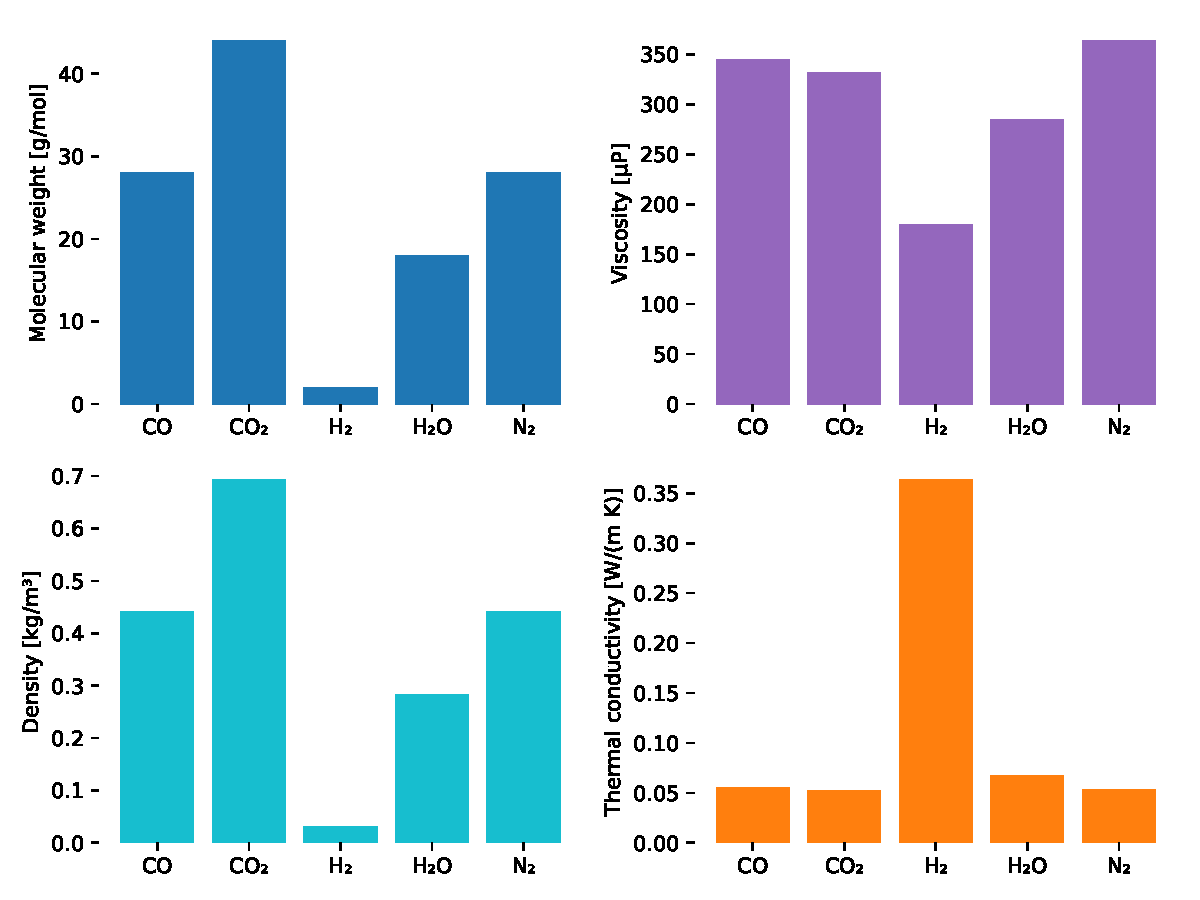
\includegraphics[width=\textwidth]{gas-properties.pdf}
    \caption{Comparison of molecular weight (MW), viscosity ($\mu$), density ($\rho$), thermal conductivity (k), heat capacity (Cp), and Prandtl number (Pr) for each gas at 101,325 Pa and 773.15 K (500$^\circ$C).}
    \label{fig:gas-properties}
\end{figure}

Properties for molecular weight, viscosity, and density for the gas mixtures investigated in this paper are shown in Figure \ref{fig:mix-properties}. Similar to the individual gas properties, the mixture properties were calculated at 101,325 Pa and 773.15 K (500$^\circ$C). The fraction of each gas in the mixture is given by the values shown at the top of each column in the figure. For example, the hydrogen and nitrogen mixture is comprised of 80\% hydrogen and 20\% nitrogen which is labeled as $0.8 + 0.2$. As expected, the carbon dioxide mixture is the heaviest in terms of molecular weight and density.

\begin{figure}[H]
    \centering
    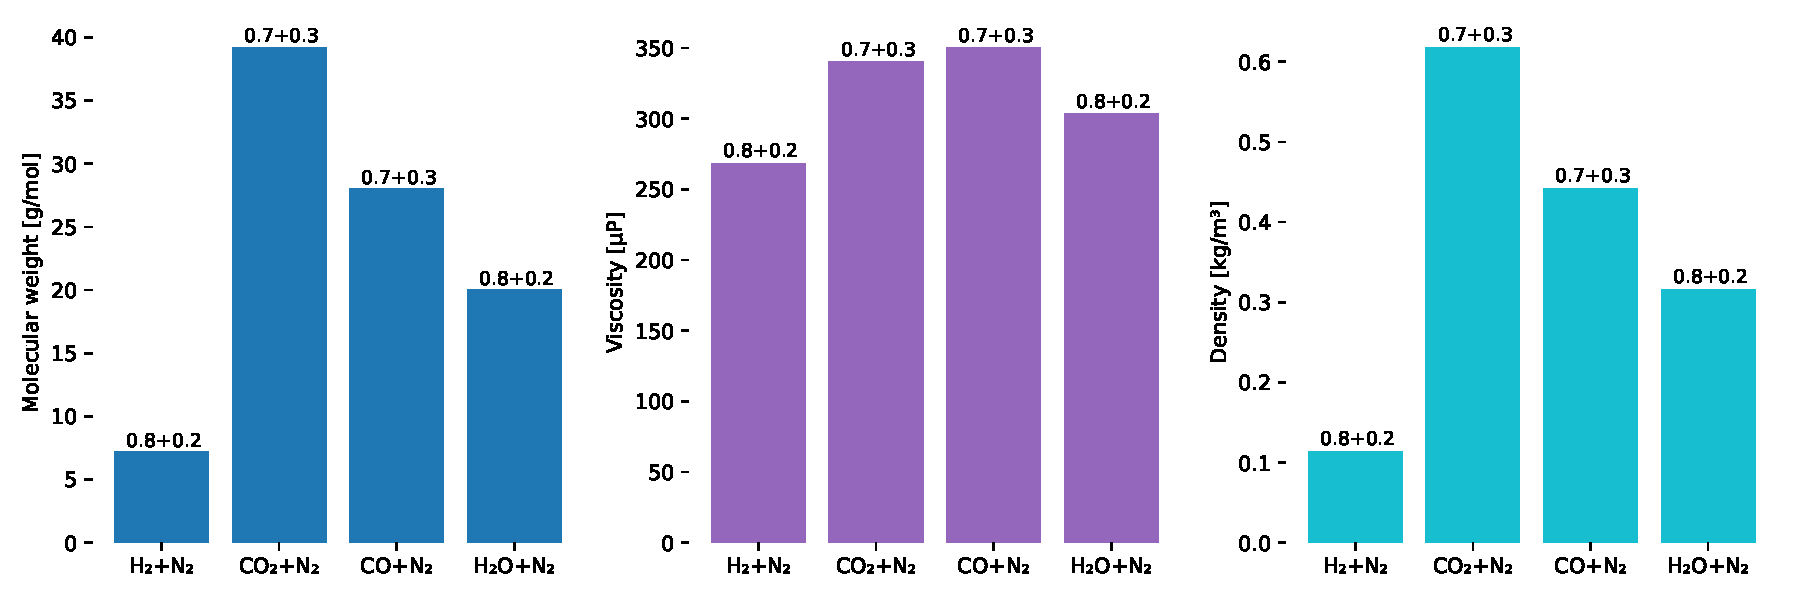
\includegraphics[width=\textwidth]{mix-properties.pdf}
    \caption{Comparison of gas mixture properties for molecular weight, viscosity, and density at 101,325 Pa and 773.15 K. Fraction of each gas component is shown at the top of each column.}
    \label{fig:mix-properties}
\end{figure}

\subsection{Fluidization effects}

Minimum fluidization velocity (Umf) of the bed material for the different fluidization gases is presented in Figure \ref{fig:gas-umf}. The hydrogen gas requires about twice the gas velocity to fluidize the sand bed compared to the nitrogen gas.

\begin{figure}[H]
    \centering
    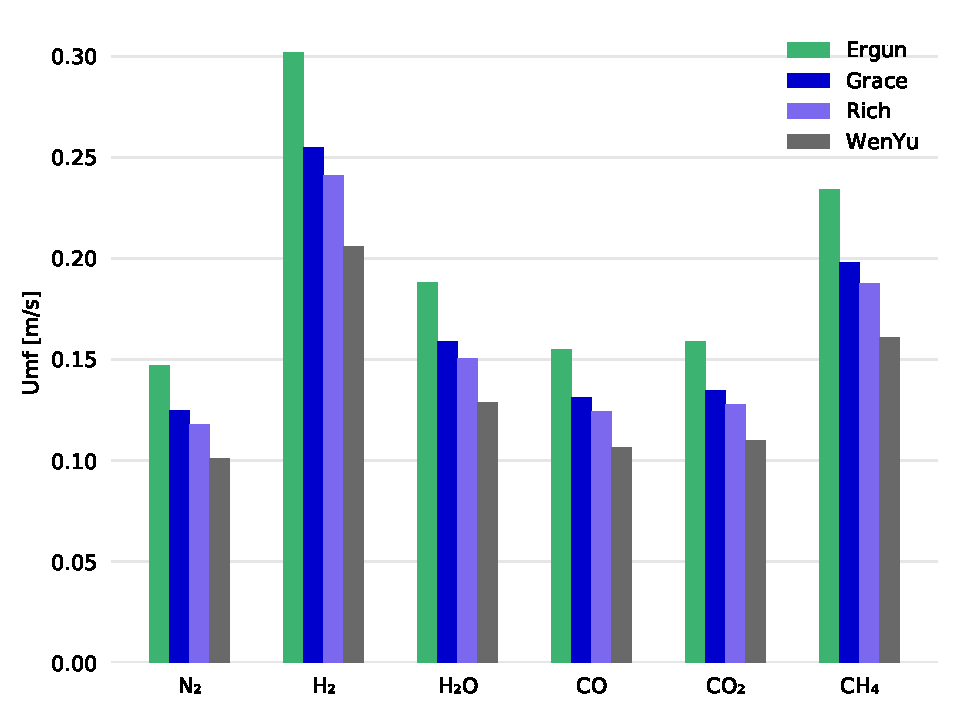
\includegraphics[width=0.8\textwidth]{gas-umf.pdf}
    \caption{Comparison of minimum fluidization velocity (Umf) for different fluidization gases. Values calculated with the Ergun, Grace, Richardson, and Wen and Yu correlations.}
    \label{fig:gas-umf}
\end{figure}

\subsection{Evaluation of the kinetic scheme}

The Di Blasi kinetics were put to use in a batch reactor model to investigate the time scales associated with the reaction mechanisms. Figure \ref{fig:batch-blasi} is an overview of the biomass conversion and product yields using the Di Blasi kinetics in a batch reactor at 773.15 K (500$^\circ$C). At this temperature, without the effects of secondary reactions, the kinetics offer a maximum achievable tar yield of 78\% within 5 seconds. However, if secondary reactions occur during the entire pyrolysis process then a maximum tar yield of only 53\% is possible. The Di Blasi kinetics suggest that minimizing the extent of secondary reactions is critical to producing the maximum possible tar yield.

A range of reaction temperatures were applied to the Di Blasi kinetics in the batch reactor model as shown in Figure \ref{fig:batch-blasi-temps}. The kinetics suggest that temperature has a neglible effect on primary tar yield but effects of secondary reactions are more pronounced. When secondary reactions occur during the entire pyrolysis process, maximum tar yields are realized at higher temperatures but with shorter residence times. These results suggest that if secondary reactions are minimized then temperature should not have a drastic effect on tar yield.

\begin{figure}[H]
    \centering
    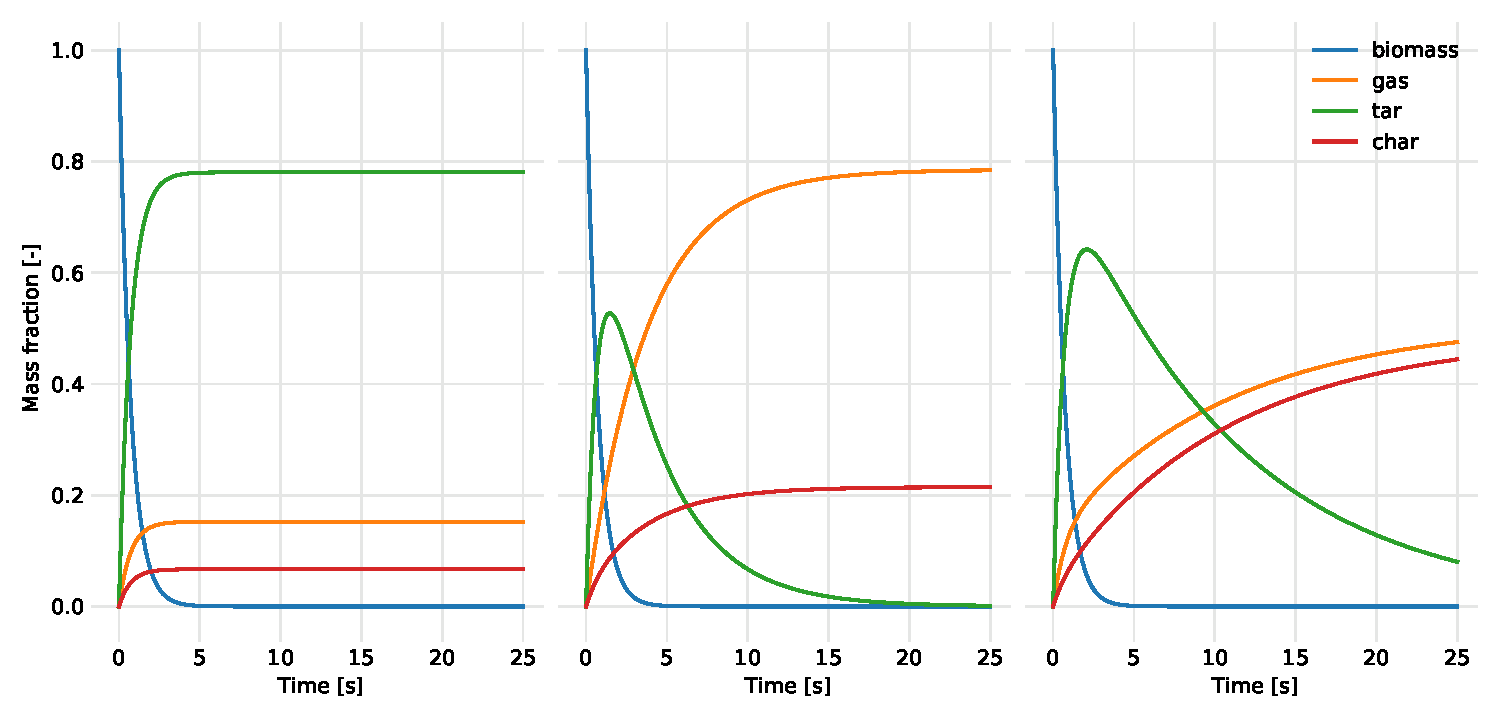
\includegraphics[width=\textwidth]{batch-blasi.pdf}
    \caption{Biomass conversion and product yields in a batch reactor model at 773.15 K (500$^\circ$C) according to the Di Blasi kinetic reactions. Results shown for primary reactions only (left) along with primary and secondary reactions (right).}
    \label{fig:batch-blasi}
\end{figure}

\begin{figure}[H]
    \centering
    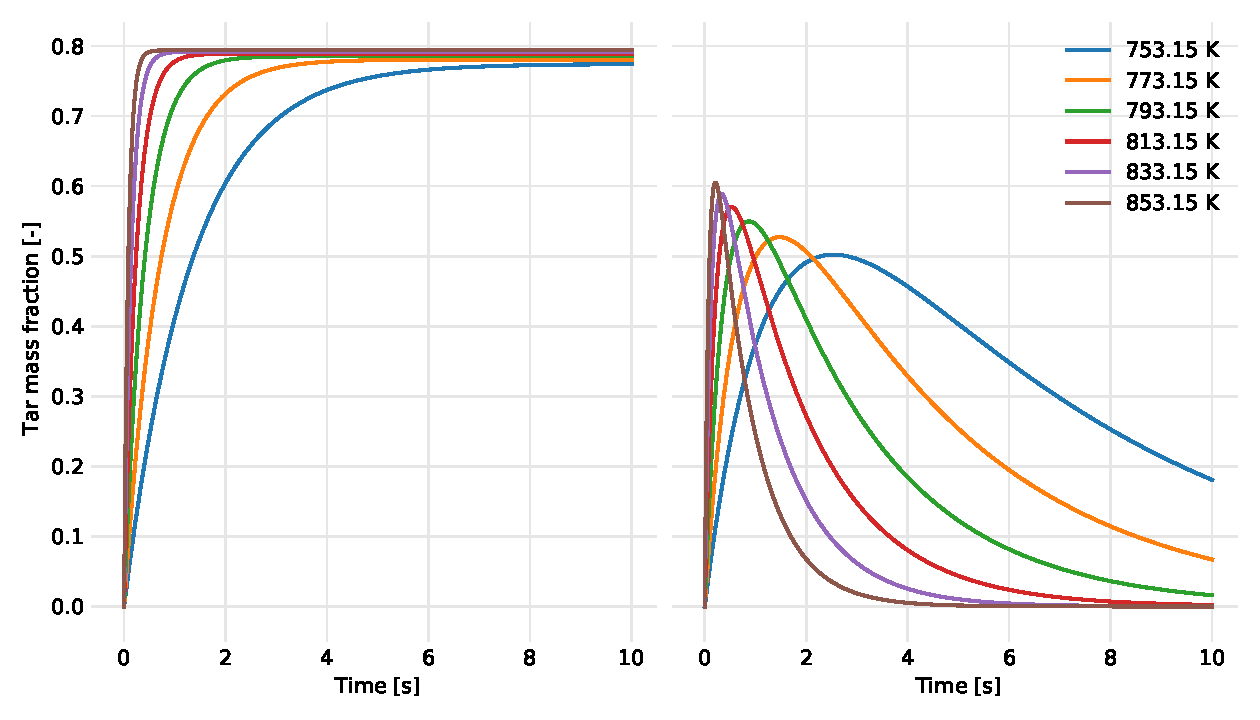
\includegraphics[width=\textwidth]{batch-blasi-temps.pdf}
    \caption{Tar yields for reaction temperatures of 753.15--853.15 K (480--580$^\circ$C) using the Di Blasi kinetics in a batch reactor model. Results shown for primary tar (left) along with primary and secondary tar (right).}
    \label{fig:batch-blasi-temps}
\end{figure}

\subsection{Solid and gas residence times}

Here.


\section{Conclusion}

Here.

\section{Source code}

Python models used to generate results for this article are available on the CCPC GitHub at \url{https://github.com/ccpcode} in the X repository. Functionality provided by the Chemics package was used for gas properties and various fluidization calculations. See the Chemics documentation at \url{https://chemics.github.io} for more information.

\printbibliography

\end{document}
